\begin{lmrarticle}%
{О пяти свойствах булевых функций}{Образцов~О.\,О., Примеров~П.\,П.}
\TwoAuthor%
{Образцов Орест Орестович}%
    {Кафедра примеров и образцов}{obrazcov\_oo@emsu.ru}%
{Примеров Петр Петрович}%
    {Кафедра шаблонов и трафаретов}{primerov\_pp@cs.msu.ru}

% Другие примеры:
%
% \OneAuthor%
% {Образцов Орест Орестович}%
%   {Эмский университет}{obrazcov\_oo@emsu.ru}%
%
% \ThreeAuthor%
% {Образцов Орест Орестович}%
%    {Кафедра примеров и образцов}{obrazcov\_oo@emsu.ru}%
% {Примеров Петр Петрович, Трафаретов Тимофей Тимофеевич}%
%    {Юмский университет}{primerov\_pp@yumsu.ru, trafaretov\_tt@yumsu.ru}

Это "--- пример оформления файла статьи. Сами правила оформления содержатся в
файле \texttt{lmr21\_guide.pdf}. Пример ссылок на статьи~[1,\,2,\,3],
диссертацию~[4], книгу~[5]. Обратите внимание на оформление ссылки~[3] на
статью с четырьмя и более авторами. Ссылки на статьи ставятся вручную.
\begin{figure}[ht]
\centering
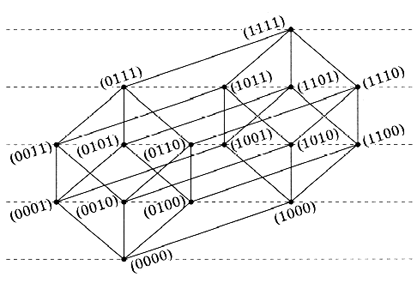
\includegraphics[width=0.6\textwidth]{bcube}
\caption{Слои булевого куба.}
\label{fi:bcube}
\end{figure}

% Раздел можно задать командой \paragraph{Название раздела}
\paragraph{Название раздела.}
Предусмотрено применение команд как использующих глобальную систему
нумерации, так и вариантов этих команд со звёздочкой, которые её не используют.
Например, ссылка на рисунок~\ref{fi:bcube} сгенерирована автоматически, а на
рисунок~2 "--- проставлена вручную, при этом в первом случае для задания
подписи к рисунку используется команда \verb|\caption|, а во втором "---
команда
\verb|\caption*|.
\begin{figure*}[ht]
\centering
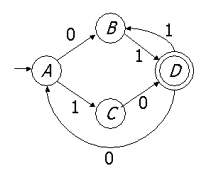
\includegraphics[width=5cm]{smach}
\caption*{Рис.~2: Пример инициального автомата.}
\end{figure*}

% Для вёрстки абзацев с переполнением строк можно
% воспользоваться окружением sloppypar
\begin{sloppypar}
Для создания выключных формул надо пользоваться окружениями \texttt
{equation}, \texttt {gather}, \texttt {multline} и др. подобными им, а также их
вариантами со звёздочкой, которые не проставляют номер формулы. При этом не
следует задавать выключные формулы с использованием команды \verb|$$|,
в~крайнем случае для этого можно воспользоваться командами \verb|\[|, \verb|\]|
(не рекомендуется). Например:
\end{sloppypar}
\begin{equation}
\label{eq:stdbase}
[\{x \&y, x \vee y, {\bar x}\}] = P_2.
\end{equation}
Для нумерации формул вручную можно воспользоваться окружением со звёздочкой и
командой~\verb|\eqno|, при этом ссылка~(2) на такую формулу также проставляется
вручную:
\begin{equation*}
\label{eq:polbase}
[\{x \oplus y, x \& y, 1, 0 \}] = P_2. \eqno{(2)}
\end{equation*}
Тезисы не должны содержать нумерованых формул, на которые нет ссылок в тексте.

% Иногда требуется, чтобы TeX сверстал параграф на одну строку короче.
% Пример показывает как этого добиться указанием команды \looseness=-1
% перед завершением следующего параграфа.
В~тексте предусмотрено использование предопределённых окружений типа
\texttt{theorem} пакета \texttt{amsthm}. Для определений, лемм, утверждений,
теорем, замечаний, следствий предлагается использовать окружения следующего
вида:\looseness=-1
\begin{definition*}
Базис $\{x \& y, x \vee y, {\bar x}\}$ называется \emph{стандартным}.
\end{definition*}
\begin{lemma}
\label{lm:nonullfn}
Формулировка леммы о ненулевой функции.
\end{lemma}
\begin{proof}
\begin{sloppy}
Доказательство леммы~\ref{lm:nonullfn}, использующее формулу~\eqref{eq:stdbase}
и заканчивающееся выключной формулой (обратите внимание на команду
\verb|\qedhere| в этом случае):
\begin{equation*}
f \neq 0. \qedhere%
\end{equation*}
\end{sloppy}
\end{proof}
\begin{statement}
\label{st:canonrep}
Формулировка устверждения о каноническом разложении функции.
\end{statement}
\begin{remark*}
Заметим, что в утверждении~\ref{st:canonrep} канонический вид единственный с
точностью до перестановки слагаемых.
\end{remark*}
\begin{theorem}
\label{th:fivebf}
Формулировка теоремы о пяти булевых функциях.
\end{theorem}
\begin{proof}
Текст доказательства теоремы~\ref{th:fivebf}.
\end{proof}
\begin{corollary*}
Формулировка следствия из теоремы~\ref{th:fivebf}.
\end{corollary*}
Все перечисленные выше окружения можно использовать как в вариантах со
звёздочкой, так и без.

Авторы выражают благодарность профессору Шаблонову~С.\,С. за постановку задачи.

Работа выполнена при поддержке РФФИ (проект \hbox{№\,15-01-12345-а}).

% Библиография создается вручную при помощи окружения lmrreferences,
% которое является разновидностью окружения enumerate
\begin{lmrreferences}
\item
Образцов~О.\,О. Некоторые свойства булевых функций~// Труды XXIV
Международной конференции <<Достижения отечественной микроэлектроники>>
(Эмск, 21--27 июня 2197\,г.). Э.~: ЗАРЯ Пресс, 2197. С.\,502--507.
\item
Образцов~О.\,О., Примеров~П.\,П., Шаблонов~Ш.\,Ш. О~свойствах
$k$"=значных функций~// Вестник Эмского государственного университета. Серия 9.
Математическая кибернетика. 2015. Т.\,1, №\,2. С.\,33--47.
\item
Некоторые свойства автоматных функций~/ О.\,О.~Образцов, П.\,П.~Примеров,
Ш.\,Ш.~Шаблонов, Т.\,Т.~Трафаретов~// Вестник Юмского государственного
университета. Серия 7.  Дискретная математика. 2016. Т.\,3, №\,1.  С.\,10--25.
\item
Примеров~П.\,П. Методы оценки сложности недоопределенных булевых
функций~: дис.  \ldots\ канд. физ.-мат. наук~: 01.01.09~/ Примеров Петр
Петрович. Юмск, 2013. 199\,с.
\item
Львовский~С.\,М. Набор и вёрстка в системе \LaTeX. М.~: МЦНМО,
2006. 448\,с.
\end{lmrreferences}
\end{lmrarticle}
